\section{Introduction}
\label{sec:Introduction}

\subsection{Overview} 
This project aims to develop a software system to visualize the architecture of artificial neural networks, or neural networks for short. Neural networks are a class of machine learning models that are inspired by the structure and function of the human brain. They are composed of a large number of interconnected processing elements, called neurons, which work together to solve complex problems. The architecture of a neural network refers to the arrangement of neurons and the connections between them. In addition to the general structure of a network, the weights and biases that control its function can provide useful insight into the inner workings of the model. The final integral parts of the neural network architecture are the activation functions that govern how data propagates through the network. An example of what one of these networks might look like can be found in Figure \ref{fig:neural_network}. Visualizing the architecture of a neural network can help students and researchers understand the structure of the model, identify potential issues, and communicate the model to others. More information on neural networks in general can be found in section \ref{sec:neural_networks}

\begin{figure}[!hb]
    \centering
    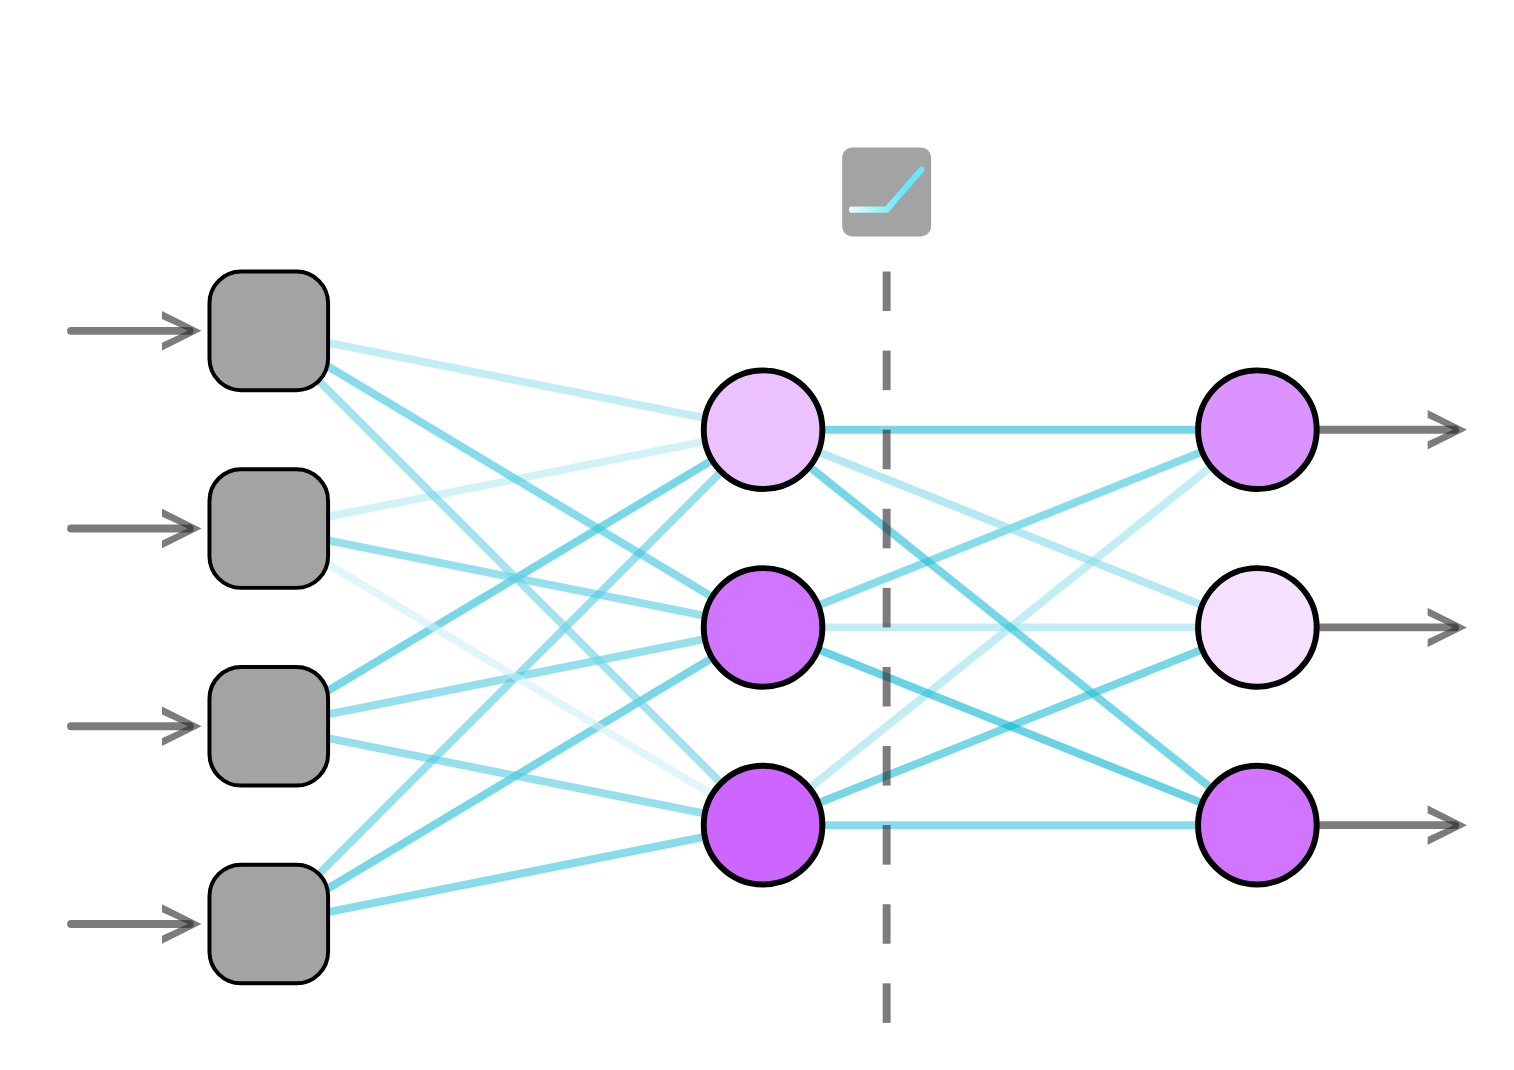
\includegraphics[width=1\textwidth]{01_introduction/res/neural_network.png}
    \caption{Example of a Neural Network}
    \label{fig:neural_network}
\end{figure}

This project developed a web application that allows users to upload pre-trained neural network models and generate visual representations of their architecture. The application supports models trained using popular machine learning frameworks such as PyTorch \cite{pytorch} and Keras \cite{keras}. The resulting graph structure is visualized in a pannable and zoomable Scalable Vector Graphic (SVG) format that shows the ordering of neurons, biases on those neurons, the weights of the connections between them and activation functions on each layer.

The application is designed to be user-friendly and accessible to a wide range of users, including students and researchers. It is implemented using modern web technologies and deployed as a web service that can be accessed from any device with an internet connection. The project was developed according to best practices in software engineering, including requirements analysis, design, implementation, testing, and deployment. The resulting application is a valuable tool for anyone working with neural networks, but in particular it will be beneficial for post-secondary educational students learning about machine learning and neural networks for the first time.

\subsection{Similar Projects}
Neural networks are a notoriously difficult concept to understand, especially for those who are newer to the field of machine learning. The architecture of a neural network is a key component of understanding how the model functions, but it can be difficult to visualize and comprehend. There are a handful to tools available for visualizing neural network architectures, but they are often limited in their scope. For example, Google's TensorBoard \cite{tensorboard} is a popular tool, but only natively supports TensorFlow and Keras models. In researching existing tools such as TensorBoard, Netron \cite{netron}, and ENNUI \cite{ennui}, it was found that none of them supported the same range of formats as NeuraViz. This project developed a user-friendly tool that is accessible to a wide range of users, including students and researchers who are new to the field of machine learning, and it supports a wider range of model formats than other offerings.

\subsection{Goals}
With an aim to solve the issues with existing tools, NeuraViz was developed with a few key goals in mind. One main goal is to support a wide range of formats and to visualize each format in a standard way. This will allow users to upload models from a variety of frameworks and see a consistent and comparable visualization of their model.

NeuraViz is also designed specifically with user-friendliness and simplicity in mind. The minimal interface focuses on the visualization of the neural networks themselves, with minimal distractions. The use of color and shape in the visualizations helps to make the network architecture more understandable at a glance, allowing the user to quickly identify neurons and connections that are the most important. Where needed, users can also zoom in or out and click on elements to see more detailed information.

Portability was another key goal of the development. Modern web technologies ensure the application is accessible from a range of devices, though it is optimized for a desktop or laptop experience. Because the application is deployed as a web application, users don't need to install software on their own machines, or even sign in to be able to use the tool. To enhance this ability further, graph representations can also be exported as raw SVG or in TikZ \cite{tikz} format for use within \LaTeX{} documents. 

\subsection{Neural Networks} \label{sec:neural_networks}
Neural networks are a type of machine learning model that are inspired by the human brain. They are made up of layers of neurons that are connected to each other. Each layer of neurons takes in a number of inputs, processes them, and then outputs a value. The value that is output is then passed to the next layer of neurons, and so on, until the final layer of neurons outputs the final result \cite{neuralnetworksanddeeplearning}.

\subsubsection{Neurons}
In an artificial neural network, neurons are the primary elements of the network that perform computations. They are organized into groups called layers, typically represented in a graph structure organized vertically so the neurons in a layer are in a sort of column. Typically, the first layer is called the input layer, and behaves differently than other layers. For this reason, input neurons are represented as grey squares in NeuraViz as opposed to the typical neurons' circles. Neurons run the computations needed for the network to process input (details can be found in "Neural Networks and Deep Learning" \cite{neuralnetworksanddeeplearning}). In general, neurons in a layer are directionally linked to all the neurons in the previous layer, and all the neurons in the next layer, with data traveling on these links from one layer to the next. These connections are represented as directed lines between the neurons in NeuraViz.

\subsubsection{Edges}
Edges are the connections between neurons in a neural network. They are the primary way that information is passed between neurons. In NeuraViz, edges are represented as directed lines between neurons. Edges also have weights, which are used in the computation to determine how important that connection is. For small enough networks, the weights can be seen by hovering over edges in NeuraViz.

\subsubsection{Activation Functions}
Activation functions are a key part of how neural networks work. They are used to determine the output of a neuron based on the inputs it receives. There are many different activation functions, but one of the most common ones is the sigmoid function. The sigmoid function takes in a number and returns a number between 0 and 1. This is useful because it allows the network to output a value that can be interpreted as a probability. In NeuraViz, activation functions are shown at the layer-level and represented as icons near the top of each layer. Hovering over these icons will show the activation function used in that layer.
